\section{Golden Rules for Cross section, decay rates, and Feynman Diagrams}
\label{sec:GoldenRulesAndDensityOfStates}

Let us consider first the decay of a particle $A$ to particles $B, C$. The probability of this process to take place can calculated as the product of two terms:
\begin{itemize}
\item Squared magnitude of the quantum mechanical (complex) amplitude for the transition $A\to B, C$, $\left|\mathcal{M}_{BC,A}\right|^2$. (For a generic initial state $i$ and final state $f$, we'll write $\mathcal{M}_{fi}$ instead of $\mathcal{M}_{BC,A}$.)
\item The density of $B, C$ momentum states that are available, called \emph{density of states}, \emph{phase space density}, or \emph{available phase space}, and often, lazily, simply \emph{phase space}. 
You might argue that there is exactly one momentum $\vec{p}_B = -\vec{p}_C$ that $B$ can have in the $A$ restframe, if we know the masses of $A, B, C$, but in reality there is always (however small) a range due to the uncertainty principle, so the number of final states, and hence the observed decay rate, is proportional to the density of states near $\vec{p}_B$. This turns out to be related to the energy release in the decay, in such a way that the larger the energy release, the bigger the density of states. This is derived in the optional \secref{sec:densityOfStates} below.
\end{itemize}

For processes such as scattering $A, B \to C, D$, we also have to take into account "how hard I try" to shoot particles $A$ and $B$ into each other. This is expressed as the luminosity $\mathcal{L}$, measured in the number of particles impingining on each other per unit volume per unit time. In order to separate the running conditions of our experiment (expressed as $\mathcal{L}$) from the physics, we use the cross section $\sigma$, defined such that 
\begin{equation}
\mathrm{rate} = \mathcal{L} \cdot \sigma
\end{equation}

For the discussion that follows it is especially important to remember that\\
\fbox{\parbox{0.99\textwidth}{
\begin{itemize}
\item $\mathcal{M}_{fi}$ represents a quantum mechanical amplitude to go from one state $i$ to another $f$. It encapsulates "the physics". $\mathcal{M}_{fi}$ is what we calculate with Feynman diagrams. $\mathcal{M}_{fi}$ is a complex number. The rate is proportional to $\left|\mathcal{M}_{fi}\right|^2$. But the fact that $\mathcal{M}_{fi}$, and the Feynman diagrams that contribute to it, are complex, matters if several complex amplitudes interfere with each other. E.g. if $\mathcal{M}_{fi}^{\mathrm{total}} = A_1 e^{i\phi_1} + A_2 e^{i\phi_2}$ (where $A_i$, $\phi_i$ are real number and $A_1 e^{i\phi_1}$ might be represented by one Feynman diagram, and $A_2 e^{i\phi_2}$ by another), then $\left|\mathcal{M}_{fi}\right|^2 = A_1^2 + A_2^2 + 2A_1 A_2 \cos(\phi_2-\phi_1)$
\item The rate at which a process happens depends also on the density of states (proportional to the magnitude of the momentum squared), and, for scattering experiments, on the luminosity
\end{itemize}
}}

\subsection{Golden Rules}
\begin{figure}
\centering
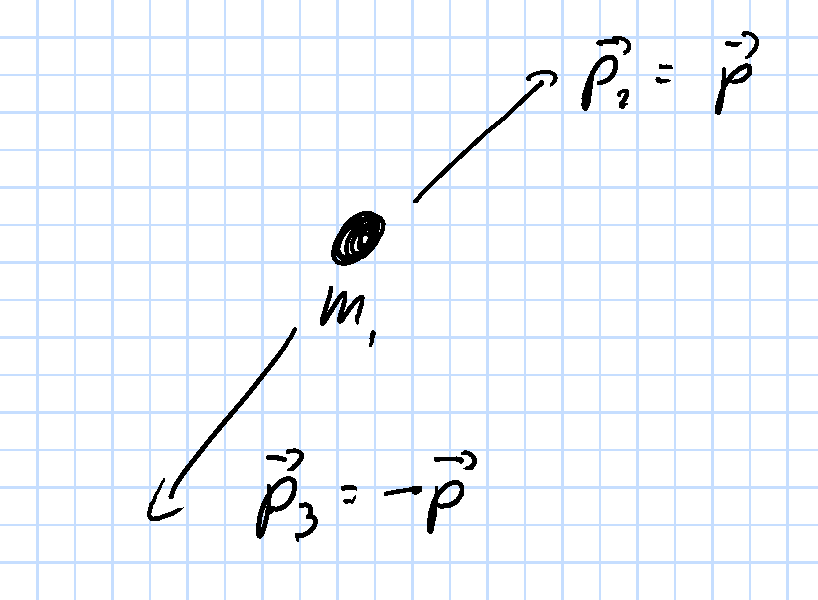
\includegraphics[width=0.4\textwidth]{fig/weak/Decay122}
\caption{Decay rate of particle $1$ into two particles (labelled $2$ and $3$) in the cm frame.\label{fig:Decay122App}}
\end{figure}
\begin{figure}
\centering
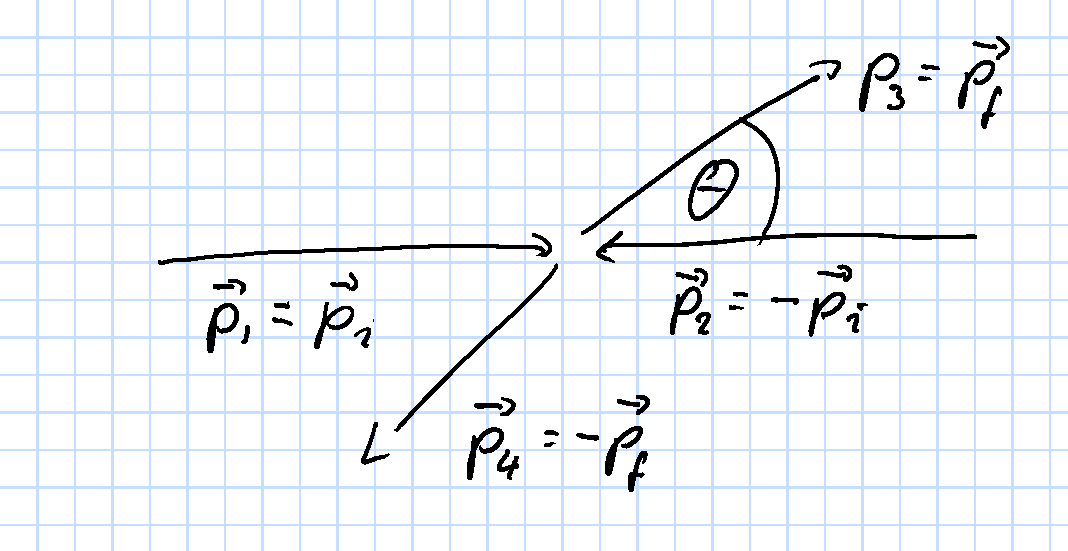
\includegraphics[width=0.7\textwidth]{fig/weak/ScatteringGeneric222}
\caption{$2$ particle to $2$ particle scattering, $1,2 \to 3,4$.\label{fig:ScatteringGeneric222App}}
\end{figure}

These golden rules relate $\mathcal{M}_{fi}$ and hence the Feynman rules to measurable quantities, taking into account phase space density. 
\paragraph{Golden Rule Decay Rates in cm frame}
(see \figref{fig:Decay122App})
Decay of particle $1$ to particles $2, 3$ in the cm frame 
\begin{equation}
\Gamma_k = \frac{S}{8\pi} \frac{|\vec{p}|}{m_1^2} \left|\mathcal{M}_{fi}\right|^2
\end{equation}
Where $m_1$ is the mass of the decaying particle, and $\vec{p}$ is momentum of one of the daughter particles, $\vec{p} = \vec{p}_2 = -\vec{p_3}$. The subscript $k$ in $\Gamma_k$ indicates that this is the \emph{partial} width for the decay to this particular final state (that we label $k$). $S$ is $1$ when the final state particles are distinguishable (as in \prt{\pi^+ \to \mu^+ \nu_{\mu}}), except when the two final state particles are identical (as in \prt{\pi^0 \to \gamma \gamma}), in which case $S = \half$.
This is what you can do with the result of this calculation:
\begin{itemize}
\item $\Gamma_k$ is the partial width of the decay of particle $1$ to particles $2, 3$.
\item If I add up all partial widths (i.e. $\Gamma_k$ calculated for all possible final states $k$, added together) I get the total width $\Gamma = \sum_k \Gamma_k$. Its inverse is the average lifetime of the particle, $\tau = 1/\Gamma$. If I start with $N_0$ particles, I expect, after time $t$ (in the particles' restframe), to find $N(t) = N_0 e^{-\Gamma t}$.
\item If we have $N$ particles, the rate at which they will decay to this given final state is $N\Gamma_k$ (note that $N$ will decrease exponentially with time, $N(t) = N_0 e^{-\Gamma t}$).
\item If I observe $n$ decays of this given type of particle, the fraction of decays $n_k$ that I expect to find in final state $k$ is $n_k/n = \Gamma_k/\Gamma$. This ratio is called the Branching Fraction.
\end{itemize}


\paragraph{Golden rule for scattering in CM frame}
This is for calculating the differential cross section for two particles in the CM frame, which have the momenta $\vec{p}_1 = \vec{p}_i$ and $\vec{p}_2 = -\vec{p}_i$, that scatter into two final state particles with momenta $\vec{p}_3 = \vec{p}_f$ and $\vec{p}_4 = -\vec{p}_f$ as illustrated in \figref{fig:ScatteringGeneric222App}:
\begin{equation}
\frac{d \sigma}{d\Omega}= \frac{S}{64\pi^2} \frac{1}{(E_1 + E_2)^2} \frac{|\vec{p}_f|}{|\vec{p}_i|} \left|\mathcal{M}_{fi}\right|^2
\end{equation}
We label the incoming particles as $1, 2$ and the outgoing as $3, 4$.
Here, $d\Omega$ is a solid angle element $d\phi\; d(\cos\theta)$. The scattering angle $\theta$ is defined relative to $\vec{p}_i$, and $\phi$ (not shown in the diagram) is the angle of rotation around the axis defined by the initial momenta (you have a choice how you define these angles, e.g. is $\theta$ the angle of $\vec{p}_3$ relative to $\vec{p}_1$ or $\vec{p}_4$ relative to $\vec{p}_1$, that's why it's always good to draw  diagram to define this). So, $\mathcal{L} \cdot \frac{d \sigma}{d\Omega}$ is proportional to the number of events per unit time that we will observe where $\vec{p}_f$ is in the direction between $\phi$ and $\phi + d\phi$ and between $\cos(\theta)$ and $\cos(\theta) + d\cos(\theta)$ when we shoot initial state particles at each other with luminosity $\mathcal{L}$. The quantity $\frac{d \sigma}{d\Omega}$ is proportional to that, but independent of the luminosity. It is measured in units of $[\mathrm{area}]^2$, usually expressed in "barn", with symbol \units{b}. One barn is approximately the size of a nucleus: $\un{1}{b} = (\un{10^{-14}}{m})^2 = \un{100}{fm^2}$. A nucleus is huge in terms of particle physics cross sections, hence the term barn (as in "your aim is so poor, you couldn't hit the broad side of a barn"). Typical cross sections we will deal with are micro, nano or pico barn. In natural units with $\hbar=c=1$, we measure distances in \units{GeV^{-1}}, and cross sections in \units{GeV^{-2}}. The conversion is $\un{1}{GeV^{-2}} = \un{0.3894}{mb}$.

The other symbols in this equation are:
\begin{itemize}
\item $E_1 + E_2$ the centre of mass energy, $E_{cm} = E_1 + E_2 = E_3 + E_4$. $E_{cm}^2$ is the same as the Lorentz invariant $s \equiv (\sum p_j)^2 = (\sum E_j)^2 - (\sum \vec{p}_j)^2$ where the sum is taken over all particles $j$ (at a given moment, so it's either all initial XOR all final state particles). $ \sqrt{s} = E_{cm}= \sqrt{\vec{p}_1^2 + m_1^2} + \sqrt{\vec{p}_2^2 + m_2^2} = \sqrt{\vec{p}_3^2 + m_2^2} + \sqrt{\vec{p}_4^2 + m_2^2}$
\item $S$ (capital $S$): This is usually simply $1$. However, if you have a final state with indistinguishable particles, such as $e^- e^-$, it is $\half$.
\end{itemize}
In most cases, the cross section is symmetric with respect to rotations around $\phi$. However, with polarised beams (where the spin of the initial state particles has a certain direction) $\phi$ might matter.

\subsection{Density of States}
\label{sec:densityOfStates}
In this section we want to count the number different states with (nearly) the same momentum. This is important for calculating decay rates. The more states there are available, the higher the rate, in fact the rate should be directly proportional to the number of states.

 Consider standing waves in a cubic box with side length $L$ and volume $V=L^3$. The boundary conditions for standing waves lead to the following conditions:
\begin{equation}
 p_x L = n_x 2\pi,\;\;
 p_y L = n_y 2\pi,\;\;
 p_z L = n_z 2\pi
\end{equation}
 where $n_{xyz}$ are integers. For a large volume the discrete set of
 momenta approach a continuum and the number of states between $N$
 and $N+\dx{N}$ is:
\begin{equation}
 \dx{N} = \dx{n_x}\dx{n_y}\dx{n_z}
        = \frac{1}{(2\pi)^3} L^3 \dx{p_x}\dx{p_y}\dx{p_z}
        = \frac{V}{(2\pi)^3} \dIII{p}
\end{equation}
So there are is one state in each volume of size $\frac{V}{(2\pi)^3}$ in momentum space. In terms of the magnitude of the momentum $|\vec{p}|$, we get
\begin{equation}
\dx{N} = \frac{V}{(2\pi)^3} 4\pi \vec{p}^2 d|\vec{p}|
\end{equation}
And for the energy, using $E^2 = p^2 + m^2$ and consequently $E\dx{E} = p\dx{p}$
\begin{equation}
\dx{N} = \frac{V}{(2\pi)^3} 4\pi |\vec{p}| E d|\vec{E}|
\end{equation}

In the end, the overall volume will not matter, in any practical calculation it will be cancelled by a corresponding $1/V$. 

We remember:
\begin{equation}
\frac{\dx{N}}{d|\vec{p}|} \propto |p|^2
\end{equation}
where $\vec{p}$ is the momentum of a final state particle.
Note that for two particle final states, the momentum of particle $1$ determines the momentum of particle $2$, so only one such factor applies.

\paragraph{Some remarks on the approach taken above:}
Due to Heisenberg's uncertainty principle, the  momentum is never exactly known, so it makes sense to count the number of momentum states accessible to a final state, despite the kinematic constraints imposed by the particle masses. In practice, rather than actually counting how many states are within $\Delta p$,
(given by the uncertainty principle and the size of the box we considered), 
we used the density of states at a given momentum value $\vec{p}$. This is similar to the way in which we use the mass density of a solid body. There we define a smooth function $\rho(x,y,z)$ that describes the mass density, although strictly speaking, a solid body is never smooth, it's made of atoms and nuclei, etc - but we simply average over this lumpiness of matter. For the density of states in momentum space, we use the same approach - while the momenta in the box are discrete, we approximate their distribution with a smooth function. And when we take the limit that the box size goes to infinity (which we did implicitly, as in practice the box size cancels in all equations, so this step is trivial), this approximation becomes almost exact.
